
\section*{Problem 1: Redshifts}
This problem concerns determining redshifts using photometric techniques with filters to identify the Lyman break. At the rest-frame Lyman limit, $\lambda_0 = 912 \, \text{\AA}$\footnote{where $\lambda_0$ is the rest frame wavelength.}, the flux drops to nearly zero due to absorption by stellar atmospheres and the interstellar medium (ISM) causing a step like feature. This is the basis of the ``dropout technique.'' However, at high $z$ this feature can be confused with absorption by the intergalactic medium (IGM), which affects the spectrum over the range $912 \, \text{\AA} < \lambda_0 < 1216 \, \text{\AA}$. The Lyman series corresponds to electronic transitions in hydrogen where electrons fall to the ground state ($n=1$). 

The photometric technique is inherently less precise than spectroscopic redshifts, which are obtained by taking a full spectrum and fitting actual spectral lines. However, it is much cheaper and faster. This method relies on fitting template spectra to the observed data through the filters used.

\subsection*{A.}
We estimate a photometric redshift using relative fluxes (magnitudes) from different filters (Figure \ref{tab:filter_deltamag}). By comparing the template spectrum and filter responses in the video, we find $z \sim 4.6$ (Figure \ref{fig:photometric_z}).

\begin{figure}[H]
    \centering
    % Table on the left
    \begin{minipage}{0.45\linewidth}
        \centering
        \label{tab:filter_deltamag}
        \begin{tabular}{c c}
            \hline
            Filter & $\Delta$ mag \\
            \hline
            $b$ & No Flux \\
            $v$ & 1.5 \\
            $i$ & 0.1 \\
            $z$ & 0.0 \\
            \hline
        \end{tabular}
        \caption{Photometric magnitude differences by filter.}
    \end{minipage}%
    \hfill
    % Figure on the right
    \begin{minipage}{0.45\linewidth}
        \centering
        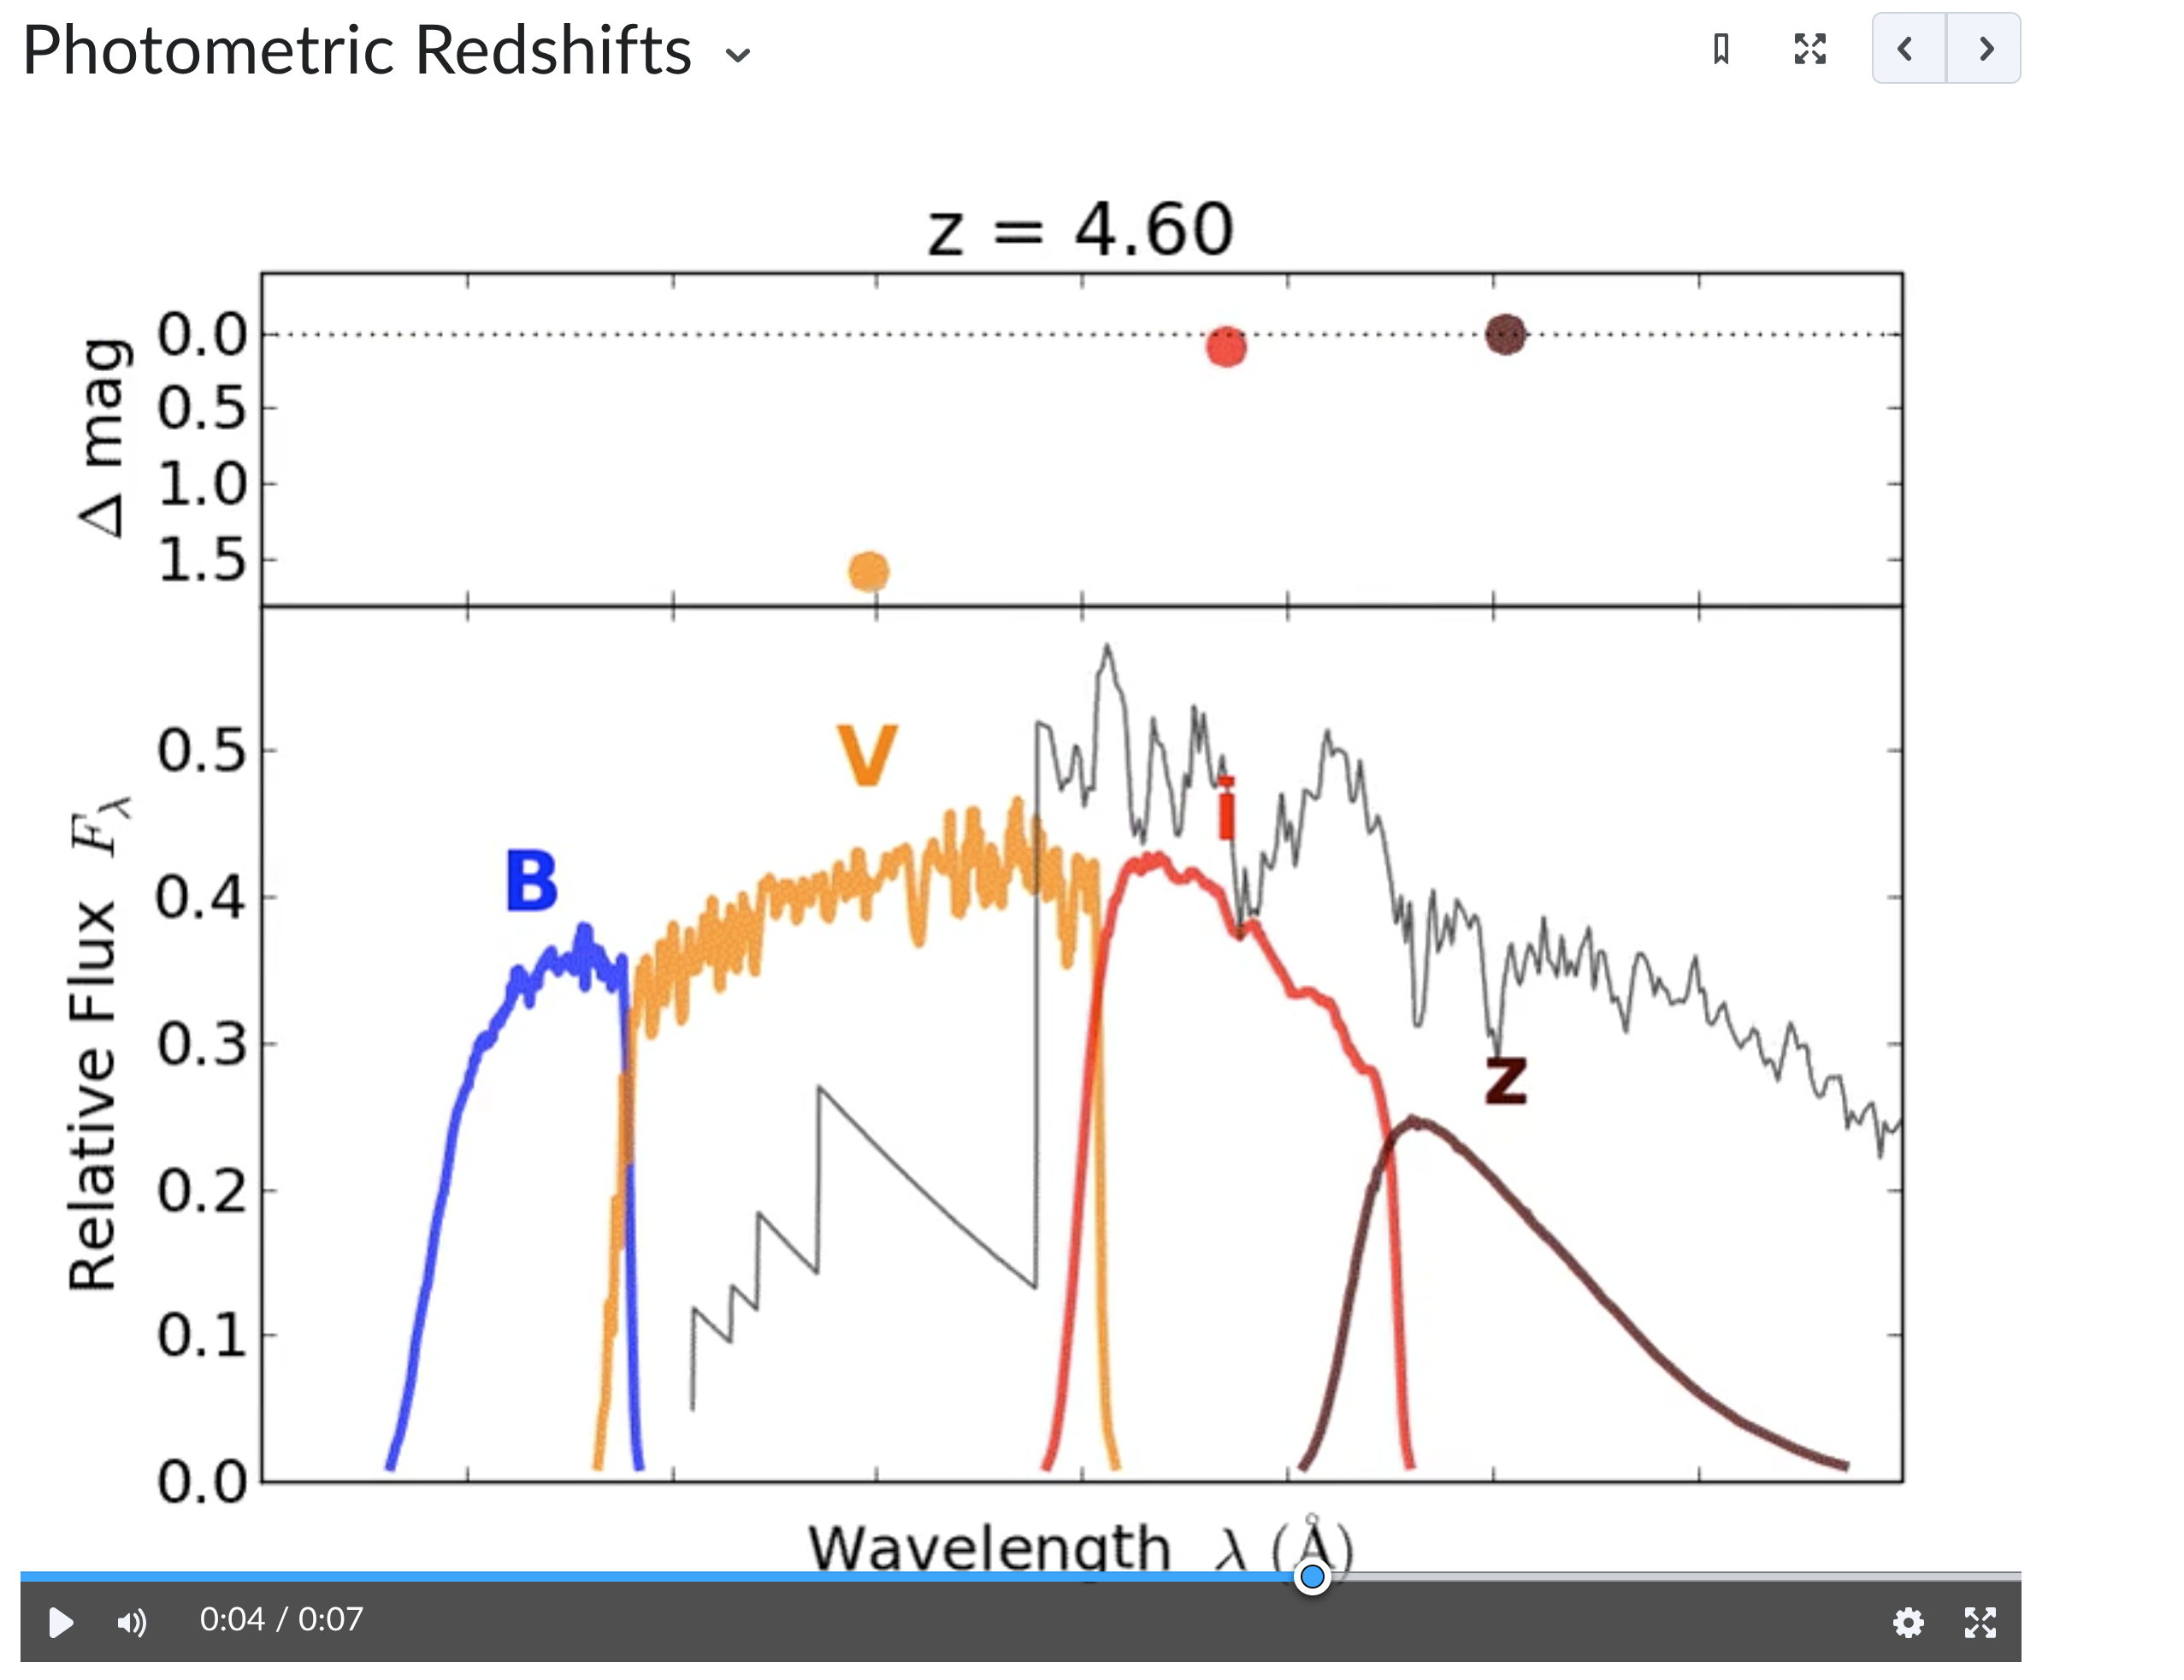
\includegraphics[width=\linewidth]{images/maxfine_phy644_problemset_1_q1_redshift.png}
        \caption{Screen shot of the photometric $z$ simulator, from \url{https://mycourses2.mcgill.ca/d2l/le/content/802628/viewContent/8637994/View}}
        \label{fig:photometric_z}
    \end{minipage}
\end{figure}




\subsection*{B.}
This time we are asked to look at Figure 1 of the homework (not reproduced), and and reflect on what redshifts can be most cleanly identified with the Lyman dropout technique before it gets confused with absorption from the IGM.  

Using the filter response, we can eyeball when the Lyman break $z$, and IGM absorption $z$, at the egde of the filters.  Using this I think, below $z \sim 6$, photometric $z$ are alright because the Lyman break moves through the optical bands.  

Beyond $z \sim 6-7$, it starts to get hard / degeneracy with IGM absorption. (Excluding effects of dusty galaxies).







